\batchmode

\documentclass[english]{article}
\RequirePackage{ifthen}


\usepackage{babel}
\usepackage{longtable}
\usepackage{html}
\usepackage{times}
\usepackage{graphicx}
\usepackage{hyperref}
\usepackage[T1]{fontenc}
\textwidth 6.5in
\textheight 8.5in

\addtolength{\oddsidemargin}{-.75in}%
\providecommand{\mytitle}{\Large {\bf NUOPC Layer Reference}}%
\providecommand{\myauthors}{\large {\it Content Standards Committee (CSC) Members}}%
\providecommand{\myversion}{ESMF 8.8.0 beta snapshot} 

\setlength{\parskip}{0pt} 

\setlength{\parindent}{0pt} 

\setlength{\baselineskip}{11pt} 

\newlength{\oldparskip} 

\newlength{\oldparindent} 

\newlength{\oldbaselineskip} 
\setlongtables
\sloppy


\usepackage{xcolor}

\usepackage[]{inputenc}



\makeatletter
\AtBeginDocument{\makeatletter
\input /sandbox/esmf/src-git/src/addon/NUOPC/doc/NUOPC_refdoc.aux
\makeatother
}

\makeatletter
\count@=\the\catcode`\_ \catcode`\_=8 
\newenvironment{tex2html_wrap}{}{}%
\catcode`\<=12\catcode`\_=\count@
\newcommand{\providedcommand}[1]{\expandafter\providecommand\csname #1\endcsname}%
\newcommand{\renewedcommand}[1]{\expandafter\providecommand\csname #1\endcsname{}%
  \expandafter\renewcommand\csname #1\endcsname}%
\newcommand{\newedenvironment}[1]{\newenvironment{#1}{}{}\renewenvironment{#1}}%
\let\newedcommand\renewedcommand
\let\renewedenvironment\newedenvironment
\makeatother
\let\mathon=$
\let\mathoff=$
\ifx\AtBeginDocument\undefined \newcommand{\AtBeginDocument}[1]{}\fi
\newbox\sizebox
\setlength{\hoffset}{0pt}\setlength{\voffset}{0pt}
\addtolength{\textheight}{\footskip}\setlength{\footskip}{0pt}
\addtolength{\textheight}{\topmargin}\setlength{\topmargin}{0pt}
\addtolength{\textheight}{\headheight}\setlength{\headheight}{0pt}
\addtolength{\textheight}{\headsep}\setlength{\headsep}{0pt}
\setlength{\textwidth}{349pt}
\newwrite\lthtmlwrite
\makeatletter
\let\realnormalsize=\normalsize
\global\topskip=2sp
\def\preveqno{}\let\real@float=\@float \let\realend@float=\end@float
\def\@float{\let\@savefreelist\@freelist\real@float}
\def\liih@math{\ifmmode$\else\bad@math\fi}
\def\end@float{\realend@float\global\let\@freelist\@savefreelist}
\let\real@dbflt=\@dbflt \let\end@dblfloat=\end@float
\let\@largefloatcheck=\relax
\let\if@boxedmulticols=\iftrue
\def\@dbflt{\let\@savefreelist\@freelist\real@dbflt}
\def\adjustnormalsize{\def\normalsize{\mathsurround=0pt \realnormalsize
 \parindent=0pt\abovedisplayskip=0pt\belowdisplayskip=0pt}%
 \def\phantompar{\csname par\endcsname}\normalsize}%
\def\lthtmltypeout#1{{\let\protect\string \immediate\write\lthtmlwrite{#1}}}%
\newcommand\lthtmlhboxmathA{\adjustnormalsize\setbox\sizebox=\hbox\bgroup\kern.05em }%
\newcommand\lthtmlhboxmathB{\adjustnormalsize\setbox\sizebox=\hbox to\hsize\bgroup\hfill }%
\newcommand\lthtmlvboxmathA{\adjustnormalsize\setbox\sizebox=\vbox\bgroup %
 \let\ifinner=\iffalse \let\)\liih@math }%
\newcommand\lthtmlboxmathZ{\@next\next\@currlist{}{\def\next{\voidb@x}}%
 \expandafter\box\next\egroup}%
\newcommand\lthtmlmathtype[1]{\gdef\lthtmlmathenv{#1}}%
\newcommand\lthtmllogmath{\dimen0\ht\sizebox \advance\dimen0\dp\sizebox
  \ifdim\dimen0>.95\vsize
   \lthtmltypeout{%
*** image for \lthtmlmathenv\space is too tall at \the\dimen0, reducing to .95 vsize ***}%
   \ht\sizebox.95\vsize \dp\sizebox\z@ \fi
  \lthtmltypeout{l2hSize %
:\lthtmlmathenv:\the\ht\sizebox::\the\dp\sizebox::\the\wd\sizebox.\preveqno}}%
\newcommand\lthtmlfigureA[1]{\let\@savefreelist\@freelist
       \lthtmlmathtype{#1}\lthtmlvboxmathA}%
\newcommand\lthtmlpictureA{\bgroup\catcode`\_=8 \lthtmlpictureB}%
\newcommand\lthtmlpictureB[1]{\lthtmlmathtype{#1}\egroup
       \let\@savefreelist\@freelist \lthtmlhboxmathB}%
\newcommand\lthtmlpictureZ[1]{\hfill\lthtmlfigureZ}%
\newcommand\lthtmlfigureZ{\lthtmlboxmathZ\lthtmllogmath\copy\sizebox
       \global\let\@freelist\@savefreelist}%
\newcommand\lthtmldisplayA{\bgroup\catcode`\_=8 \lthtmldisplayAi}%
\newcommand\lthtmldisplayAi[1]{\lthtmlmathtype{#1}\egroup\lthtmlvboxmathA}%
\newcommand\lthtmldisplayB[1]{\edef\preveqno{(\theequation)}%
  \lthtmldisplayA{#1}\let\@eqnnum\relax}%
\newcommand\lthtmldisplayZ{\lthtmlboxmathZ\lthtmllogmath\lthtmlsetmath}%
\newcommand\lthtmlinlinemathA{\bgroup\catcode`\_=8 \lthtmlinlinemathB}
\newcommand\lthtmlinlinemathB[1]{\lthtmlmathtype{#1}\egroup\lthtmlhboxmathA
  \vrule height1.5ex width0pt }%
\newcommand\lthtmlinlineA{\bgroup\catcode`\_=8 \lthtmlinlineB}%
\newcommand\lthtmlinlineB[1]{\lthtmlmathtype{#1}\egroup\lthtmlhboxmathA}%
\newcommand\lthtmlinlineZ{\egroup\expandafter\ifdim\dp\sizebox>0pt %
  \expandafter\centerinlinemath\fi\lthtmllogmath\lthtmlsetinline}
\newcommand\lthtmlinlinemathZ{\egroup\expandafter\ifdim\dp\sizebox>0pt %
  \expandafter\centerinlinemath\fi\lthtmllogmath\lthtmlsetmath}
\newcommand\lthtmlindisplaymathZ{\egroup %
  \centerinlinemath\lthtmllogmath\lthtmlsetmath}
\def\lthtmlsetinline{\hbox{\vrule width.1em \vtop{\vbox{%
  \kern.1em\copy\sizebox}\ifdim\dp\sizebox>0pt\kern.1em\else\kern.3pt\fi
  \ifdim\hsize>\wd\sizebox \hrule depth1pt\fi}}}
\def\lthtmlsetmath{\hbox{\vrule width.1em\kern-.05em\vtop{\vbox{%
  \kern.1em\kern0.8 pt\hbox{\hglue.17em\copy\sizebox\hglue0.8 pt}}\kern.3pt%
  \ifdim\dp\sizebox>0pt\kern.1em\fi \kern0.8 pt%
  \ifdim\hsize>\wd\sizebox \hrule depth1pt\fi}}}
\def\centerinlinemath{%
  \dimen1=\ifdim\ht\sizebox<\dp\sizebox \dp\sizebox\else\ht\sizebox\fi
  \advance\dimen1by.5pt \vrule width0pt height\dimen1 depth\dimen1 
 \dp\sizebox=\dimen1\ht\sizebox=\dimen1\relax}

\def\lthtmlcheckvsize{\ifdim\ht\sizebox<\vsize 
  \ifdim\wd\sizebox<\hsize\expandafter\hfill\fi \expandafter\vfill
  \else\expandafter\vss\fi}%
\providecommand{\selectlanguage}[1]{}%
\makeatletter \tracingstats = 1 


\begin{document}
\pagestyle{empty}\thispagestyle{empty}\lthtmltypeout{}%
\lthtmltypeout{latex2htmlLength hsize=\the\hsize}\lthtmltypeout{}%
\lthtmltypeout{latex2htmlLength vsize=\the\vsize}\lthtmltypeout{}%
\lthtmltypeout{latex2htmlLength hoffset=\the\hoffset}\lthtmltypeout{}%
\lthtmltypeout{latex2htmlLength voffset=\the\voffset}\lthtmltypeout{}%
\lthtmltypeout{latex2htmlLength topmargin=\the\topmargin}\lthtmltypeout{}%
\lthtmltypeout{latex2htmlLength topskip=\the\topskip}\lthtmltypeout{}%
\lthtmltypeout{latex2htmlLength headheight=\the\headheight}\lthtmltypeout{}%
\lthtmltypeout{latex2htmlLength headsep=\the\headsep}\lthtmltypeout{}%
\lthtmltypeout{latex2htmlLength parskip=\the\parskip}\lthtmltypeout{}%
\lthtmltypeout{latex2htmlLength oddsidemargin=\the\oddsidemargin}\lthtmltypeout{}%
\makeatletter
\if@twoside\lthtmltypeout{latex2htmlLength evensidemargin=\the\evensidemargin}%
\else\lthtmltypeout{latex2htmlLength evensidemargin=\the\oddsidemargin}\fi%
\lthtmltypeout{}%
\makeatother
\setcounter{page}{1}
\onecolumn

% !!! IMAGES START HERE !!!


%
\providecommand{\apiStatusCompatibleVersion}[1]{This interface is backward compatible with ESMF versions starting at #1. If code using this interface compiles with any version of ESMF starting with #1, then it will compile with the current version.}%


%
\providecommand{\apiStatusModifiedSinceVersion}[1]{This interface was modified since ESMF version #1. The fact that code using this interface compiles with the current ESMF version does not guarantee that it compiles with previous versions of this interface. If user code compatibility with version #1 is desired then care must be taken to limit the use of this interface to features that were available in the #1 release. \\
Changes made after the #1 release:}%


%
\providecommand{\apiStatusCompatibleVersionExceptions}[1]{This interface is backward compatible with ESMF versions starting at #1 - {\em except those arguments indicated below}.}%


%
\providecommand{\apiStatusCompatibleException}{{\sc Status:}{\em This argument is excluded from the backward compatibility statement}.\\}%


%
\providecommand{\apiDeprecatedArg}{\sf DEPRECATED ARGUMENT!}%


%
\providecommand{\apiDeprecatedArgWithReplacement}[1]{{\bf DEPRECATED ARGUMENT!} Please use the argument {\tt #1} instead.}%


%
\providecommand{\apiDeprecatedMethodWithReplacement}[3]{{\bf DEPRECATED METHOD} as of ESMF #1. Please use {\tt #2}, section {\tt \ref{#3}} instead.}%


%
\providecommand{\apiDeprecatedClassWithTargetReleaseAndReplacement}[4]{{\bf DEPRECATED CLASS!}\\The entire #1 class has been deprecated and is scheduled for removal with ESMF #2. This includes all of the class derived types, named constants, and methods. Please use the replacment class {\tt #3}, section {\tt \ref{#4}} instead!\\}%



\setlength{\parskip}{1.5ex}%

\setlength{\parskip}{1.5ex}
\stepcounter{section}
\stepcounter{section}
\stepcounter{subsection}
\stepcounter{subsubsection}
\stepcounter{subsubsection}
{\newpage\clearpage
\lthtmlpictureA{tex2html_wrap401}%
\scalebox{0.6}{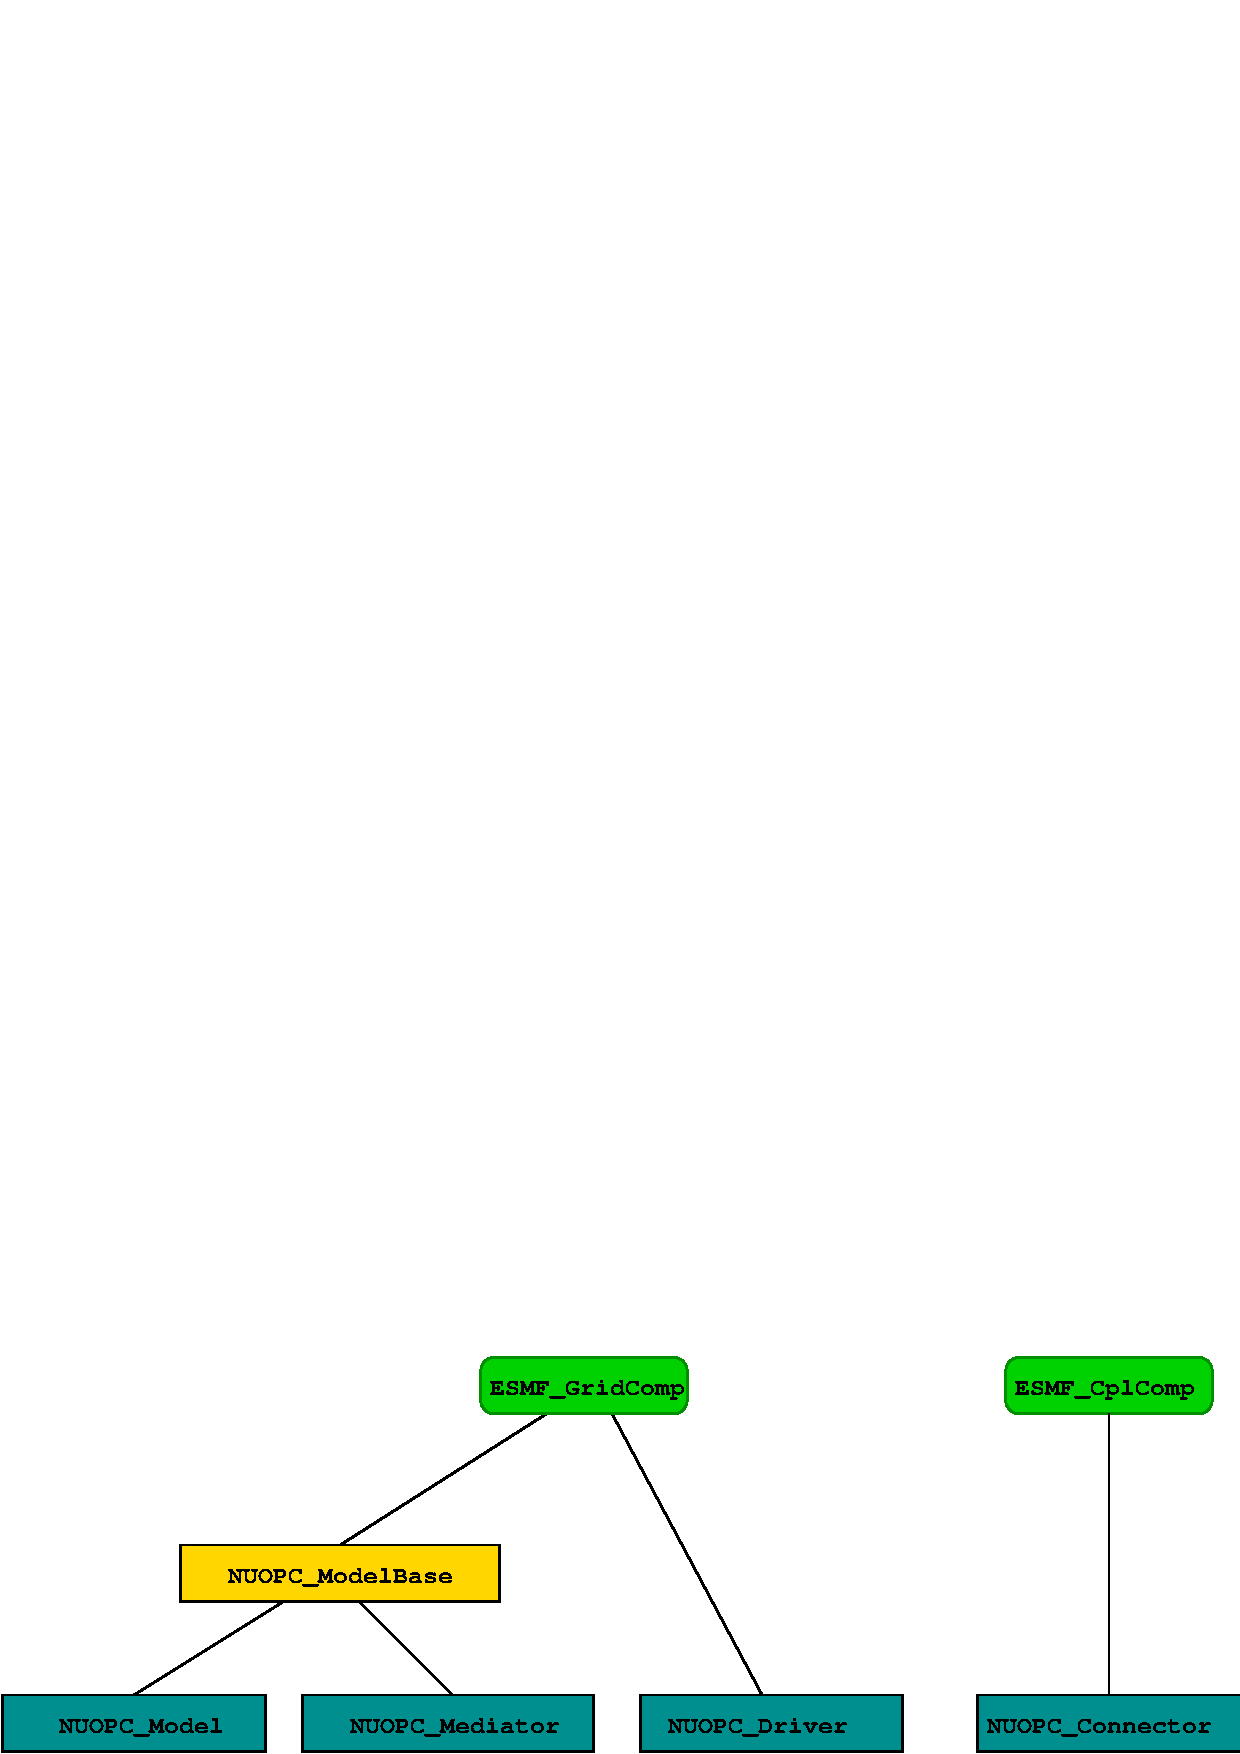
\includegraphics{NUOPC_GC}}%
\lthtmlpictureZ
\lthtmlcheckvsize\clearpage}

\stepcounter{subsection}
\stepcounter{subsubsection}
\stepcounter{subsubsection}


\setlength{\oldparskip}{\parskip}%

\setlength{\oldparskip}{\parskip}


\setlength{\parskip}{1.5ex}%

\setlength{\parskip}{1.5ex}


\setlength{\oldparindent}{\parindent}%

\setlength{\oldparindent}{\parindent}


\setlength{\parindent}{0pt}%

\setlength{\parindent}{0pt}


\setlength{\oldbaselineskip}{\baselineskip}%

\setlength{\oldbaselineskip}{\baselineskip}


\setlength{\baselineskip}{11pt}%

\setlength{\baselineskip}{11pt}


\setlength{\parskip}{\oldparskip}%

\setlength{\parskip}{\oldparskip}


\setlength{\parindent}{\oldparindent}%

\setlength{\parindent}{\oldparindent}


\setlength{\baselineskip}{\oldbaselineskip}%

\setlength{\baselineskip}{\oldbaselineskip}
\stepcounter{subsection}
\stepcounter{subsubsection}
{\newpage\clearpage
\lthtmlinlinemathA{tex2html_wrap_inline705}%
$>>>$%
\lthtmlinlinemathZ
\lthtmlcheckvsize\clearpage}

{\newpage\clearpage
\lthtmlinlinemathA{tex2html_wrap_inline707}%
$<<<$%
\lthtmlinlinemathZ
\lthtmlcheckvsize\clearpage}

\stepcounter{subsubsection}
\stepcounter{subsubsection}
\stepcounter{subsubsection}
\stepcounter{subsubsection}
\stepcounter{subsubsection}
\stepcounter{subsection}
\stepcounter{subsubsection}
\stepcounter{subsubsection}
\stepcounter{subsubsection}
\stepcounter{subsubsection}
\stepcounter{subsubsection}
\stepcounter{subsubsection}
\stepcounter{subsubsection}
\stepcounter{subsubsection}
\stepcounter{subsubsection}
\stepcounter{subsection}
\stepcounter{subsection}
\stepcounter{subsection}
\stepcounter{subsection}
\stepcounter{section}
\stepcounter{subsection}


\setlength{\parskip}{0pt}%

\setlength{\parskip}{0pt}


\setlength{\parindent}{0pt}%

\setlength{\parindent}{0pt}


\setlength{\baselineskip}{11pt}%

\setlength{\baselineskip}{11pt}


\setlength{\oldparskip}{\parskip}%

\setlength{\oldparskip}{\parskip}


\setlength{\parskip}{1.5ex}%

\setlength{\parskip}{1.5ex}


\setlength{\oldparindent}{\parindent}%

\setlength{\oldparindent}{\parindent}


\setlength{\parindent}{0pt}%

\setlength{\parindent}{0pt}


\setlength{\oldbaselineskip}{\baselineskip}%

\setlength{\oldbaselineskip}{\baselineskip}


\setlength{\baselineskip}{11pt}%

\setlength{\baselineskip}{11pt}
\stepcounter{subsubsection}
\stepcounter{subsubsection}
\stepcounter{subsubsection}
\stepcounter{subsubsection}
\stepcounter{subsubsection}
\stepcounter{subsubsection}
\stepcounter{subsubsection}
\stepcounter{subsubsection}
\stepcounter{subsubsection}
\stepcounter{subsubsection}
\stepcounter{subsubsection}
\stepcounter{subsubsection}
\stepcounter{subsubsection}
{\newpage\clearpage
\lthtmlinlinemathA{tex2html_wrap_inline4021}%
$100s$%
\lthtmlinlinemathZ
\lthtmlcheckvsize\clearpage}

{\newpage\clearpage
\lthtmlinlinemathA{tex2html_wrap_inline4023}%
$800s$%
\lthtmlinlinemathZ
\lthtmlcheckvsize\clearpage}

{\newpage\clearpage
\lthtmlinlinemathA{tex2html_wrap_inline4033}%
$1000s$%
\lthtmlinlinemathZ
\lthtmlcheckvsize\clearpage}

{\newpage\clearpage
\lthtmlinlinemathA{tex2html_wrap_inline4037}%
$1800s$%
\lthtmlinlinemathZ
\lthtmlcheckvsize\clearpage}

\stepcounter{subsubsection}
\stepcounter{subsubsection}
\stepcounter{subsubsection}
\stepcounter{subsubsection}


\setlength{\parskip}{\oldparskip}%

\setlength{\parskip}{\oldparskip}


\setlength{\parindent}{\oldparindent}%

\setlength{\parindent}{\oldparindent}


\setlength{\baselineskip}{\oldbaselineskip}%

\setlength{\baselineskip}{\oldbaselineskip}
\stepcounter{subsection}


\setlength{\parskip}{0pt}%

\setlength{\parskip}{0pt}


\setlength{\parindent}{0pt}%

\setlength{\parindent}{0pt}


\setlength{\baselineskip}{11pt}%

\setlength{\baselineskip}{11pt}
\stepcounter{subsection}


\setlength{\parskip}{0pt}%

\setlength{\parskip}{0pt}


\setlength{\parindent}{0pt}%

\setlength{\parindent}{0pt}


\setlength{\baselineskip}{11pt}%

\setlength{\baselineskip}{11pt}


\setlength{\oldparskip}{\parskip}%

\setlength{\oldparskip}{\parskip}


\setlength{\parskip}{1.5ex}%

\setlength{\parskip}{1.5ex}


\setlength{\oldparindent}{\parindent}%

\setlength{\oldparindent}{\parindent}


\setlength{\parindent}{0pt}%

\setlength{\parindent}{0pt}


\setlength{\oldbaselineskip}{\baselineskip}%

\setlength{\oldbaselineskip}{\baselineskip}


\setlength{\baselineskip}{11pt}%

\setlength{\baselineskip}{11pt}
\stepcounter{subsubsection}


\setlength{\parskip}{\oldparskip}%

\setlength{\parskip}{\oldparskip}


\setlength{\parindent}{\oldparindent}%

\setlength{\parindent}{\oldparindent}


\setlength{\baselineskip}{\oldbaselineskip}%

\setlength{\baselineskip}{\oldbaselineskip}
\stepcounter{subsection}


\setlength{\parskip}{0pt}%

\setlength{\parskip}{0pt}


\setlength{\parindent}{0pt}%

\setlength{\parindent}{0pt}


\setlength{\baselineskip}{11pt}%

\setlength{\baselineskip}{11pt}


\setlength{\oldparskip}{\parskip}%

\setlength{\oldparskip}{\parskip}


\setlength{\parskip}{1.5ex}%

\setlength{\parskip}{1.5ex}


\setlength{\oldparindent}{\parindent}%

\setlength{\oldparindent}{\parindent}


\setlength{\parindent}{0pt}%

\setlength{\parindent}{0pt}


\setlength{\oldbaselineskip}{\baselineskip}%

\setlength{\oldbaselineskip}{\baselineskip}


\setlength{\baselineskip}{11pt}%

\setlength{\baselineskip}{11pt}
\stepcounter{subsubsection}


\setlength{\parskip}{\oldparskip}%

\setlength{\parskip}{\oldparskip}


\setlength{\parindent}{\oldparindent}%

\setlength{\parindent}{\oldparindent}


\setlength{\baselineskip}{\oldbaselineskip}%

\setlength{\baselineskip}{\oldbaselineskip}
\stepcounter{subsection}


\setlength{\parskip}{0pt}%

\setlength{\parskip}{0pt}


\setlength{\parindent}{0pt}%

\setlength{\parindent}{0pt}


\setlength{\baselineskip}{11pt}%

\setlength{\baselineskip}{11pt}


\setlength{\oldparskip}{\parskip}%

\setlength{\oldparskip}{\parskip}


\setlength{\parskip}{1.5ex}%

\setlength{\parskip}{1.5ex}


\setlength{\oldparindent}{\parindent}%

\setlength{\oldparindent}{\parindent}


\setlength{\parindent}{0pt}%

\setlength{\parindent}{0pt}


\setlength{\oldbaselineskip}{\baselineskip}%

\setlength{\oldbaselineskip}{\baselineskip}


\setlength{\baselineskip}{11pt}%

\setlength{\baselineskip}{11pt}
\stepcounter{subsubsection}
\stepcounter{subsubsection}


\setlength{\parskip}{\oldparskip}%

\setlength{\parskip}{\oldparskip}


\setlength{\parindent}{\oldparindent}%

\setlength{\parindent}{\oldparindent}


\setlength{\baselineskip}{\oldbaselineskip}%

\setlength{\baselineskip}{\oldbaselineskip}
\stepcounter{subsection}


\setlength{\oldparskip}{\parskip}%

\setlength{\oldparskip}{\parskip}


\setlength{\parskip}{1.5ex}%

\setlength{\parskip}{1.5ex}


\setlength{\oldparindent}{\parindent}%

\setlength{\oldparindent}{\parindent}


\setlength{\parindent}{0pt}%

\setlength{\parindent}{0pt}


\setlength{\oldbaselineskip}{\baselineskip}%

\setlength{\oldbaselineskip}{\baselineskip}


\setlength{\baselineskip}{11pt}%

\setlength{\baselineskip}{11pt}
\stepcounter{subsubsection}
\stepcounter{subsubsection}
\stepcounter{subsubsection}
\stepcounter{subsubsection}
\stepcounter{subsubsection}
\stepcounter{subsubsection}
\stepcounter{subsubsection}
\stepcounter{subsubsection}
\stepcounter{subsubsection}
\stepcounter{subsubsection}
\stepcounter{subsubsection}
\stepcounter{subsubsection}
\stepcounter{subsubsection}
\stepcounter{subsubsection}
\stepcounter{subsubsection}
\stepcounter{subsubsection}
\stepcounter{subsubsection}
\stepcounter{subsubsection}
\stepcounter{subsubsection}
\stepcounter{subsubsection}
\stepcounter{subsubsection}
\stepcounter{subsubsection}
\stepcounter{subsubsection}
\stepcounter{subsubsection}
\stepcounter{subsubsection}
\stepcounter{subsubsection}
\stepcounter{subsubsection}
\stepcounter{subsubsection}
\stepcounter{subsubsection}
\stepcounter{subsubsection}
\stepcounter{subsubsection}
\stepcounter{subsubsection}
\stepcounter{subsubsection}
\stepcounter{subsubsection}
\stepcounter{subsubsection}
\stepcounter{subsubsection}
\stepcounter{subsubsection}
\stepcounter{subsubsection}
\stepcounter{subsubsection}
\stepcounter{subsubsection}
\stepcounter{subsubsection}
\stepcounter{subsubsection}
\stepcounter{subsubsection}
\stepcounter{subsubsection}
\stepcounter{subsubsection}


\setlength{\parskip}{\oldparskip}%

\setlength{\parskip}{\oldparskip}


\setlength{\parindent}{\oldparindent}%

\setlength{\parindent}{\oldparindent}


\setlength{\baselineskip}{\oldbaselineskip}%

\setlength{\baselineskip}{\oldbaselineskip}
\stepcounter{subsection}


\setlength{\oldparskip}{\parskip}%

\setlength{\oldparskip}{\parskip}


\setlength{\parskip}{1.5ex}%

\setlength{\parskip}{1.5ex}


\setlength{\oldparindent}{\parindent}%

\setlength{\oldparindent}{\parindent}


\setlength{\parindent}{0pt}%

\setlength{\parindent}{0pt}


\setlength{\oldbaselineskip}{\baselineskip}%

\setlength{\oldbaselineskip}{\baselineskip}


\setlength{\baselineskip}{11pt}%

\setlength{\baselineskip}{11pt}
\stepcounter{subsubsection}
\stepcounter{subsubsection}
\stepcounter{subsubsection}
\stepcounter{subsubsection}
\stepcounter{subsubsection}
\stepcounter{subsubsection}
\stepcounter{subsubsection}
\stepcounter{subsubsection}


\setlength{\parskip}{\oldparskip}%

\setlength{\parskip}{\oldparskip}


\setlength{\parindent}{\oldparindent}%

\setlength{\parindent}{\oldparindent}


\setlength{\baselineskip}{\oldbaselineskip}%

\setlength{\baselineskip}{\oldbaselineskip}
\stepcounter{subsection}


\setlength{\oldparskip}{\parskip}%

\setlength{\oldparskip}{\parskip}


\setlength{\parskip}{1.5ex}%

\setlength{\parskip}{1.5ex}


\setlength{\oldparindent}{\parindent}%

\setlength{\oldparindent}{\parindent}


\setlength{\parindent}{0pt}%

\setlength{\parindent}{0pt}


\setlength{\oldbaselineskip}{\baselineskip}%

\setlength{\oldbaselineskip}{\baselineskip}


\setlength{\baselineskip}{11pt}%

\setlength{\baselineskip}{11pt}
\stepcounter{subsubsection}
\stepcounter{subsubsection}
\stepcounter{subsubsection}
\stepcounter{subsubsection}
\stepcounter{subsubsection}
\stepcounter{subsubsection}
\stepcounter{subsubsection}
\stepcounter{subsubsection}


\setlength{\parskip}{\oldparskip}%

\setlength{\parskip}{\oldparskip}


\setlength{\parindent}{\oldparindent}%

\setlength{\parindent}{\oldparindent}


\setlength{\baselineskip}{\oldbaselineskip}%

\setlength{\baselineskip}{\oldbaselineskip}
\stepcounter{subsection}


\setlength{\oldparskip}{\parskip}%

\setlength{\oldparskip}{\parskip}


\setlength{\parskip}{1.5ex}%

\setlength{\parskip}{1.5ex}


\setlength{\oldparindent}{\parindent}%

\setlength{\oldparindent}{\parindent}


\setlength{\parindent}{0pt}%

\setlength{\parindent}{0pt}


\setlength{\oldbaselineskip}{\baselineskip}%

\setlength{\oldbaselineskip}{\baselineskip}


\setlength{\baselineskip}{11pt}%

\setlength{\baselineskip}{11pt}
\stepcounter{subsubsection}
\stepcounter{subsubsection}
\stepcounter{subsubsection}
\stepcounter{subsubsection}
\stepcounter{subsubsection}
\stepcounter{subsubsection}
\stepcounter{subsubsection}
\stepcounter{subsubsection}
\stepcounter{subsubsection}
\stepcounter{subsubsection}
\stepcounter{subsubsection}
\stepcounter{subsubsection}
\stepcounter{subsubsection}
\stepcounter{subsubsection}
\stepcounter{subsubsection}
\stepcounter{subsubsection}
\stepcounter{subsubsection}
\stepcounter{subsubsection}
\stepcounter{subsubsection}
\stepcounter{subsubsection}
\stepcounter{subsubsection}
\stepcounter{subsubsection}
\stepcounter{subsubsection}
\stepcounter{subsubsection}
\stepcounter{subsubsection}
\stepcounter{subsubsection}
\stepcounter{subsubsection}
\stepcounter{subsubsection}
\stepcounter{subsubsection}
\stepcounter{subsubsection}
\stepcounter{subsubsection}
\stepcounter{subsubsection}
\stepcounter{subsubsection}


\setlength{\parskip}{\oldparskip}%

\setlength{\parskip}{\oldparskip}


\setlength{\parindent}{\oldparindent}%

\setlength{\parindent}{\oldparindent}


\setlength{\baselineskip}{\oldbaselineskip}%

\setlength{\baselineskip}{\oldbaselineskip}
\stepcounter{subsection}


\setlength{\oldparskip}{\parskip}%

\setlength{\oldparskip}{\parskip}


\setlength{\parskip}{1.5ex}%

\setlength{\parskip}{1.5ex}


\setlength{\oldparindent}{\parindent}%

\setlength{\oldparindent}{\parindent}


\setlength{\parindent}{0pt}%

\setlength{\parindent}{0pt}


\setlength{\oldbaselineskip}{\baselineskip}%

\setlength{\oldbaselineskip}{\baselineskip}


\setlength{\baselineskip}{11pt}%

\setlength{\baselineskip}{11pt}
\stepcounter{subsubsection}
\stepcounter{subsubsection}
\stepcounter{subsubsection}
\stepcounter{subsubsection}
\stepcounter{subsubsection}


\setlength{\parskip}{\oldparskip}%

\setlength{\parskip}{\oldparskip}


\setlength{\parindent}{\oldparindent}%

\setlength{\parindent}{\oldparindent}


\setlength{\baselineskip}{\oldbaselineskip}%

\setlength{\baselineskip}{\oldbaselineskip}


\setlength{\parskip}{1.5ex}%

\setlength{\parskip}{1.5ex}
\stepcounter{section}
\stepcounter{subsection}
\stepcounter{subsection}
\stepcounter{subsection}
\stepcounter{subsection}
\stepcounter{subsection}
\stepcounter{section}
\stepcounter{subsection}
\stepcounter{subsection}
\stepcounter{section}
{\newpage\clearpage
\lthtmlpictureA{tex2html_wrap12251}%
\scalebox{0.6}{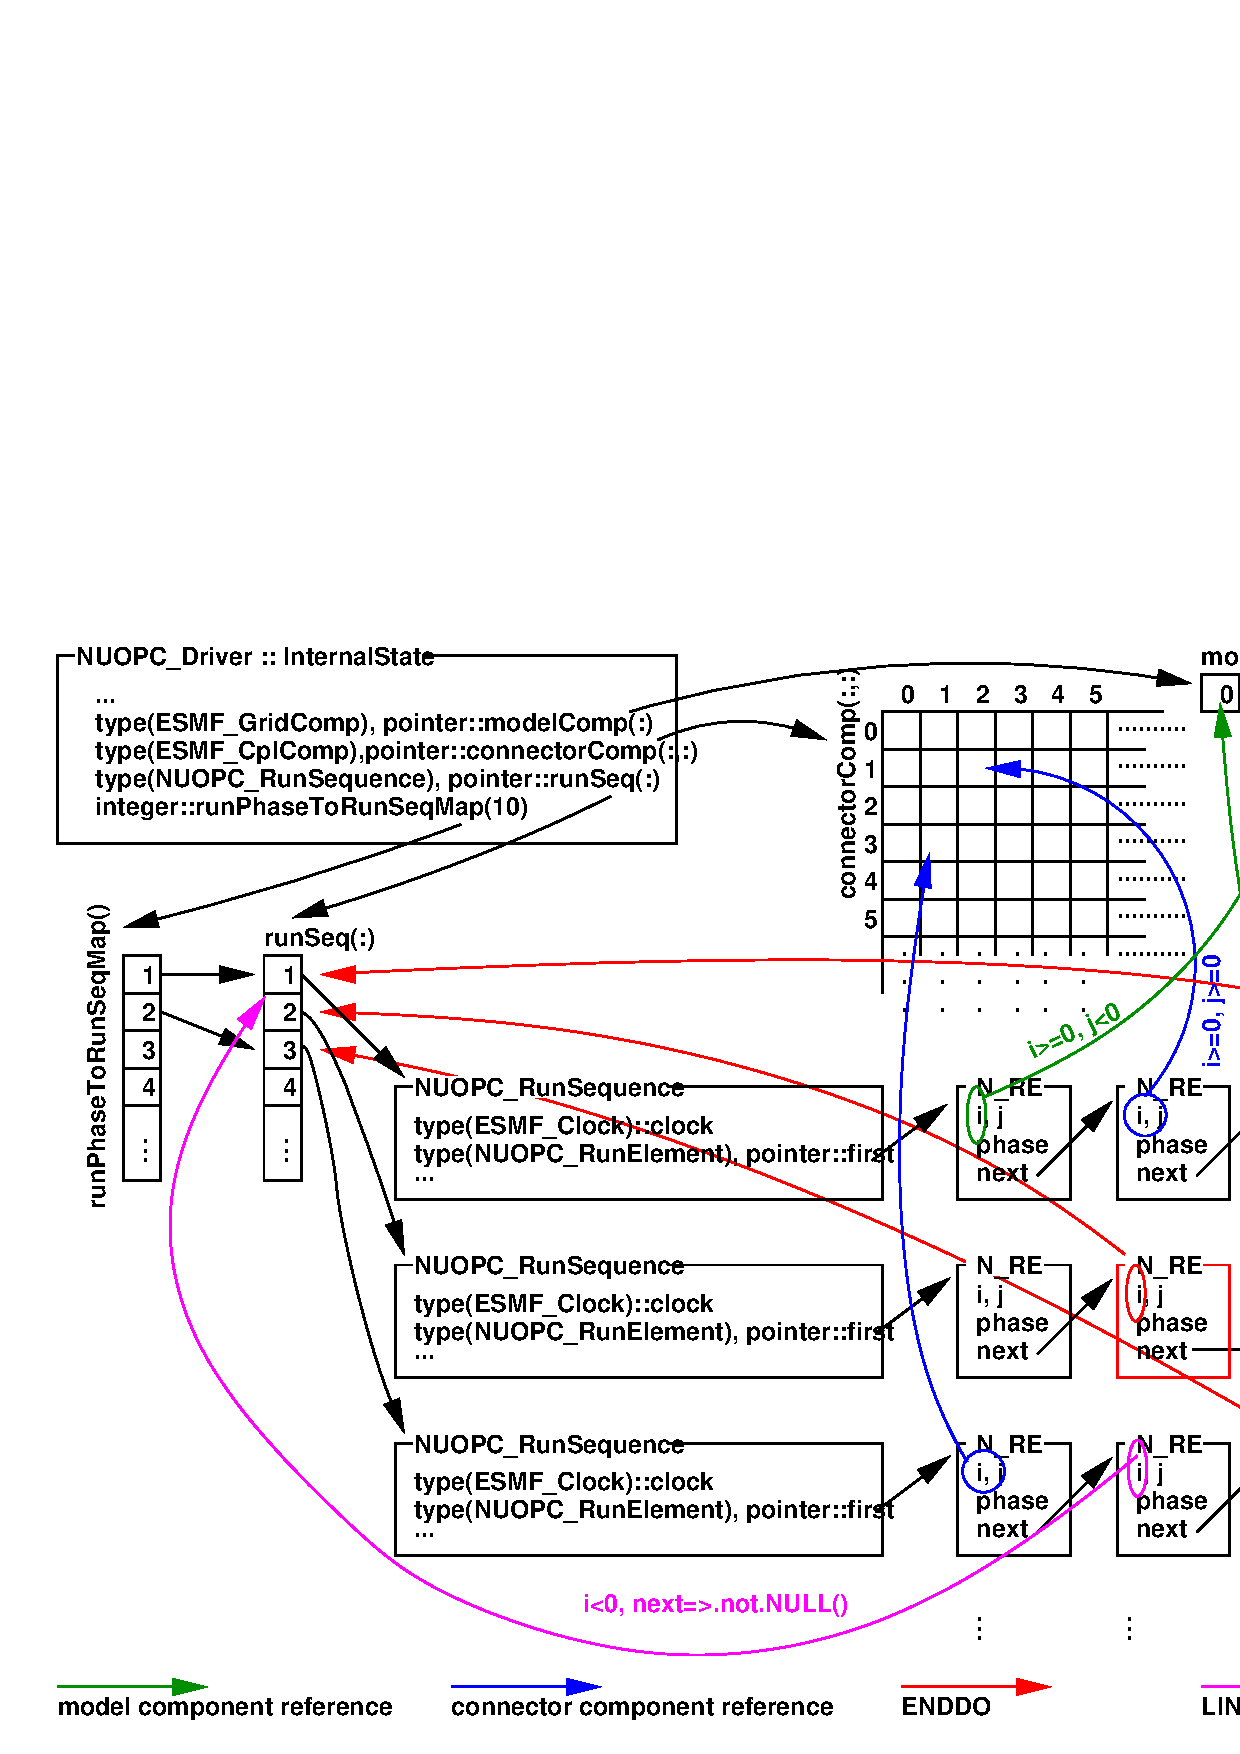
\includegraphics{NUOPC_RunSequence}}%
\lthtmlpictureZ
\lthtmlcheckvsize\clearpage}

\stepcounter{section}
\stepcounter{subsection}
\stepcounter{subsection}
\stepcounter{subsection}
\stepcounter{subsubsection}
\stepcounter{subsubsection}
\stepcounter{subsubsection}
\stepcounter{subsubsection}
\stepcounter{subsubsection}
\stepcounter{subsubsection}
\stepcounter{subsubsection}
\stepcounter{subsection}
\stepcounter{subsection}

\end{document}
